%%%%%%%%%%%%%%%%%%%%%%%%%%%%%%%%%%%%%%%%%
% Artigo - Cadernos de Visualização de Dados (template do prof. Gustavo)
% Projeto: city_bike_analysis (Citi Bike NYC, 2024)
% Versão com 5 figuras (3 páginas)
%%%%%%%%%%%%%%%%%%%%%%%%%%%%%%%%%%%%%%%%%

%% CONFIGURAÇÃO
\documentclass[10pt, a4paper, twocolumn]{article}
%%%%%%%%%%%%%%%%%%%%%%%%%%%%%%%%%%%%%%%%%
% ARQUIVO DE CONFIGURAÇÃO PARA O TEMPLATE DE ARTIGOS DO 
% 'CADERNOS DE VISUALIZAÇÃO DE DADOS'
% http://ci.ufpb.br
%
% Adaptado por @Gustavo Oliveira.
%
% 
% This file originates from:
% http://www.LaTeXTemplates.com
%
% Authors:
% Frits Wenneker
% Vel (vel@LaTeXTemplates.com)
%
% License:
% CC BY-NC-SA 3.0 (http://creativecommons.org/licenses/by-nc-sa/3.0/)
%
%%%%%%%%%%%%%%%%%%%%%%%%%%%%%%%%%%%%%%%%%

%----------------------------------------------------------------------------------------
%	PACKAGES AND OTHER DOCUMENT CONFIGURATIONS
%----------------------------------------------------------------------------------------

% CI logo colors

\usepackage[brazil]{babel} % English language hyphenation

\usepackage{microtype} % Better typography

\usepackage{amsmath,amsfonts,amsthm,bm} % Math packages for equations

\usepackage[svgnames]{xcolor} % Enabling colors by their 'svgnames'
\definecolor{blueCI}{rgb}{0.086, 0.65, 1.0}
\definecolor{blackCI}{rgb}{0.086, 0.13,0.16}

\usepackage[hang, small, labelfont=bf, up, textfont=it]{caption} % Custom captions under/above tables and figures

\usepackage{booktabs} % Horizontal rules in tables

\usepackage{lastpage} % Used to determine the number of pages in the document (for "Page X of Total")

\usepackage{graphicx} % Required for adding images

\usepackage{enumitem} % Required for customising lists
\setlist{noitemsep} % Remove spacing between bullet/numbered list elements

\usepackage{sectsty} % Enables custom section titles
\allsectionsfont{\color{blackCI}} % Change the font of all section commands (Helvetica)

\usepackage[colorlinks,linkcolor=blueCI,urlcolor=blueCI,citecolor=blueCI]{hyperref}
\urlstyle{same} % same font as text

\usepackage{lipsum}

%----------------------------------------------------------------------------------------
%	MARGINS AND SPACING
%----------------------------------------------------------------------------------------

\usepackage{geometry} % Required for adjusting page dimensions

\geometry{
	top=1cm, % Top margin
	bottom=1.5cm, % Bottom margin
	left=2cm, % Left margin
	right=2cm, % Right margin
	includehead, % Include space for a header
	includefoot, % Include space for a footer
	%showframe, % Uncomment to show how the type block is set on the page
}

\setlength{\columnsep}{7mm} % Column separation width

%----------------------------------------------------------------------------------------
%	FONTS
%----------------------------------------------------------------------------------------

\usepackage[T1]{fontenc} % Output font encoding for international characters
\usepackage[utf8]{inputenc} % Required for inputting international characters

\usepackage[sfdefault,scaled=.85]{FiraSans}
\usepackage{newtxsf}
%----------------------------------------------------------------------------------------
%	HEADERS AND FOOTERS
%----------------------------------------------------------------------------------------

\usepackage{fancyhdr} % Needed to define custom headers/footers
\pagestyle{fancy} % Enables the custom headers/footers

\renewcommand{\headrulewidth}{0.0pt} % No header rule
\renewcommand{\footrulewidth}{0.4pt} % Thin footer rule

\renewcommand{\sectionmark}[1]{\markboth{#1}{}} % Removes the section number from the header when \leftmark is used

%\nouppercase\leftmark % Add this to one of the lines below if you want a section title in the header/footer

% Headers
\lhead{} % Left header
\chead{\textit{\thetitle}} % Center header - currently printing the article title
\rhead{} % Right header

% Footers
\lfoot{} % Left footer
\cfoot{} % Center footer
\rfoot{\footnotesize \thepage}% de \pageref*{LastPage}} % Right footer, "Page 1 of 2"

\fancypagestyle{firstpage}{ % Page style for the first page with the title
	\fancyhf{}
	\renewcommand{\footrulewidth}{0pt} % Suppress footer rule
}

%----------------------------------------------------------------------------------------
%	TITLE SECTION
%----------------------------------------------------------------------------------------

\newcommand{\authorstyle}[1]{{\large\color{blueCI}#1}} % Authors style (Helvetica)

\newcommand{\institution}[1]{{\footnotesize\usefont{OT1}{phv}{m}{sl}\color{blackCI}#1}} % Institutions style (Helvetica)

\usepackage{titling} % Allows custom title configuration

\newcommand{\HorRule}{\color{blueCI}\rule{\linewidth}{1pt}} % Defines the horizontal rule around the title

\newcommand{\TITFONT}{20}
\pretitle{
	\vspace{-30pt} % Move the entire title section up
	\HorRule\vspace{10pt} % Horizontal rule before the title
	\fontsize{\TITFONT}{1.2\TITFONT}\usefont{OT1}{phv}{b}{n}\selectfont % Helvetica
	\color{blackCI} % Text colour for the title and author(s)
}

\posttitle{\par\vskip 15pt} % Whitespace under the title

\preauthor{} % Anything that will appear before \author is printed

\postauthor{ % Anything that will appear after \author is printed
	\vspace{3pt} % Space before the rule
    \flushright{\footnotesize Universidade Federal da Paraíba \\ Cadernos de Visualização de Dados\\ \url{ci.ufpb.br}}
	\par\HorRule % Horizontal rule after the title
	\vspace{10pt} % Space after the title section
}

%----------------------------------------------------------------------------------------
%	ABSTRACT
%----------------------------------------------------------------------------------------

\usepackage{lettrine} % Package to accentuate the first letter of the text (lettrine)
\usepackage{fix-cm}	% Fixes the height of the lettrine

\newcommand{\initial}[1]{ % Defines the command and style for the lettrine
	\lettrine[lines=2,findent=4pt,nindent=0pt]{% Lettrine takes up 3 lines, the text to the right of it is indented 4pt and further indenting of lines 2+ is stopped
		\color{blueCI}% Lettrine colour
		{#1}% The letter
	}{}%
}

\usepackage{xstring} % Required for string manipulation

\newcommand{\lettrineabstract}[1]{\color{blackCI}
	\StrLeft{#1}{1}[\firstletter] % Capture the first letter of the abstract for the lettrine
	\initial{\firstletter}\textbf{\StrGobbleLeft{#1}{1}} % Print the abstract with the first letter as a lettrine and the rest in bold
}

%----------------------------------------------------------------------------------------
%	BIBLIOGRAPHY
%----------------------------------------------------------------------------------------

\renewcommand{\refname}{\normalsize{Referências}}

\usepackage[backend=bibtex,style=authoryear,natbib=true]{biblatex} % Use the bibtex backend with the authoryear citation style (which resembles APA)

\addbibresource{refs.bib} % The filename of the bibliography

\usepackage[autostyle=true]{csquotes} % Required to generate language-dependent quotes in the bibliography
 % arquivo de configuração do professor (copiar sem alterar)

% as figuras ficam na pasta plots/
\graphicspath{{plots/}}

% permite figuras largas ocuparem mais espaço da página
\renewcommand{\dbltopfraction}{0.9}
\renewcommand{\dblfloatpagefraction}{0.6}
\setcounter{dbltopnumber}{3}
\setcounter{totalnumber}{5}

%% IDENTIFICAÇÃO
%----------------------------------------------------------------------------------------
\title{Como Nova York pedala: sazonalidade e assimetria espaço-temporal no Citi Bike (2024)}

\author{
	\authorstyle{Tiago Brito\textsuperscript{1}, José Lima\textsuperscript{1}, Rafael Lima\textsuperscript{2}, Guilherme Rocha\textsuperscript{2}} \\
	\textsuperscript{1}\institution{Ciência da Computação, UFPB}\\
	\textsuperscript{2}\institution{Ciência de Dados e Inteligência Artificial, UFPB}\\
}

\date{9 de novembro de 2026}
%----------------------------------------------------------------------------------------

\begin{document}

\maketitle
\thispagestyle{firstpage}

%	RESUMO
%----------------------------------------------------------------------------------------
\lettrineabstract{%
Analisamos 6,88 milhões de viagens do Citi Bike, em Nova York, comparando janeiro (inverno, mês de baixa) e setembro (fim de verão, mês de alta) de 2024. Mostramos como a sazonalidade muda o volume e o perfil dos usuários, como as bicicletas elétricas dominam a frota e como o ritmo pendular dos dias úteis esvazia e lota estações de Manhattan.
}

%	CONTEÚDO
%----------------------------------------------------------------------------------------

\section*{Introdução}

O Citi Bike é o maior sistema de bicicletas compartilhadas da América do Norte, com mais de 2.000 estações em Manhattan, Brooklyn, Queens e Bronx. Sistemas assim sofrem de assimetria direcional: em certos horários, regiões inteiras ficam sem bicicletas (déficit), enquanto centros de trabalho ficam sem docas livres (superávit). Entender quando, onde e por quem o sistema é usado ajuda a planejar a rede. Respondemos a quatro perguntas: (i) como o clima altera volume e perfil dos usuários; (ii) quanto a frota elétrica é preferida; (iii) como o ritmo diário distingue dias úteis de fins de semana; (iv) onde e quando surgem os gargalos.

\section*{Dados e método}

Escolhemos janeiro e setembro de 2024 por serem extremos sazonais do sistema: janeiro, em pleno inverno, é o mês de menor movimento do ano, e setembro, no fim do verão, é o de maior. Comparar os dois permite ver como o uso muda entre o regime mais fraco e o mais forte. Usamos os registros públicos de viagens do Citi Bike \citep{citibike}, com horário de saída e chegada, estações de origem e destino, coordenadas, tipo de bicicleta e tipo de usuário. Removemos viagens iniciadas fora do mês de análise, com duração fora de 1 a 1.440 minutos e com coordenadas fora da área de Nova York. As séries horárias foram normalizadas pelo número de dias de cada regime (úteis, fins de semana e feriados), para não distorcer a comparação entre meses. O processamento foi feito em Python, com pandas \citep{pandas} e matplotlib \citep{matplotlib}. As escolhas visuais seguem a literatura de visualização \citep{tufte1983,cleveland1984,wilke2019,ware2012,berinato2016}: títulos que declaram o achado, rotulagem direta e uma paleta própria para cada variável.

\section*{Resultados}

\subsection*{Sazonalidade e perfil}

O volume salta de 1,88 milhão de viagens em janeiro para 4,98 milhões em setembro (+165\%). Os membros crescem 136\%, mas os usuários casuais quintuplicam (+401\%), e sua fatia vai de 11,0\% para 20,8\% (Figura \ref{fig:rv1}). Mesmo no frio, o uso por assinantes se mantém: o sistema funciona como transporte cotidiano.

\begin{figure*}[t]
	\centering
	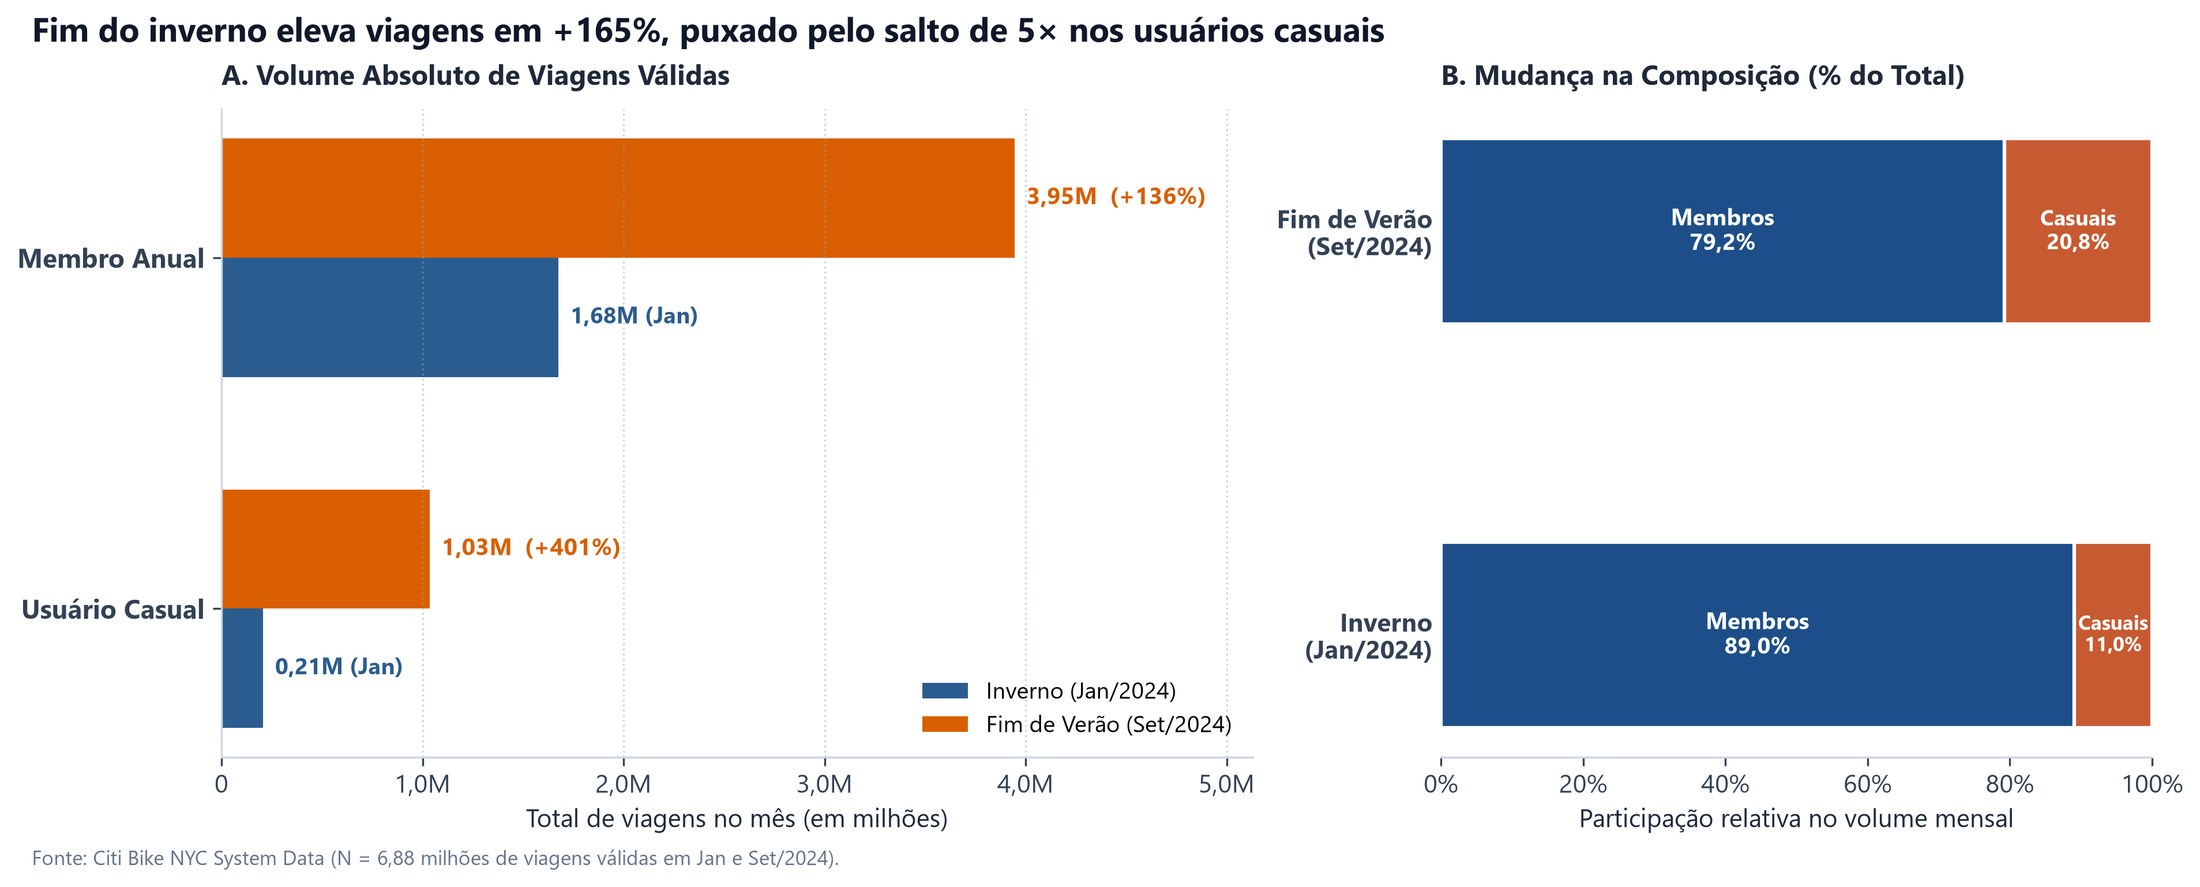
\includegraphics[width=0.9\textwidth]{rv1_sazonalidade_perfil.jpg}
	\caption{Volume de viagens por mês e perfil de usuário.}
	\label{fig:rv1}
\end{figure*}

\subsection*{Preferência de frota}

As bicicletas elétricas respondem por 62,8\% a 76,2\% das viagens em todos os recortes. A preferência é maior entre usuários casuais: 76,2\% em janeiro e 72,3\% em setembro (Figura \ref{fig:rv2}).

\begin{figure*}[t]
	\centering
	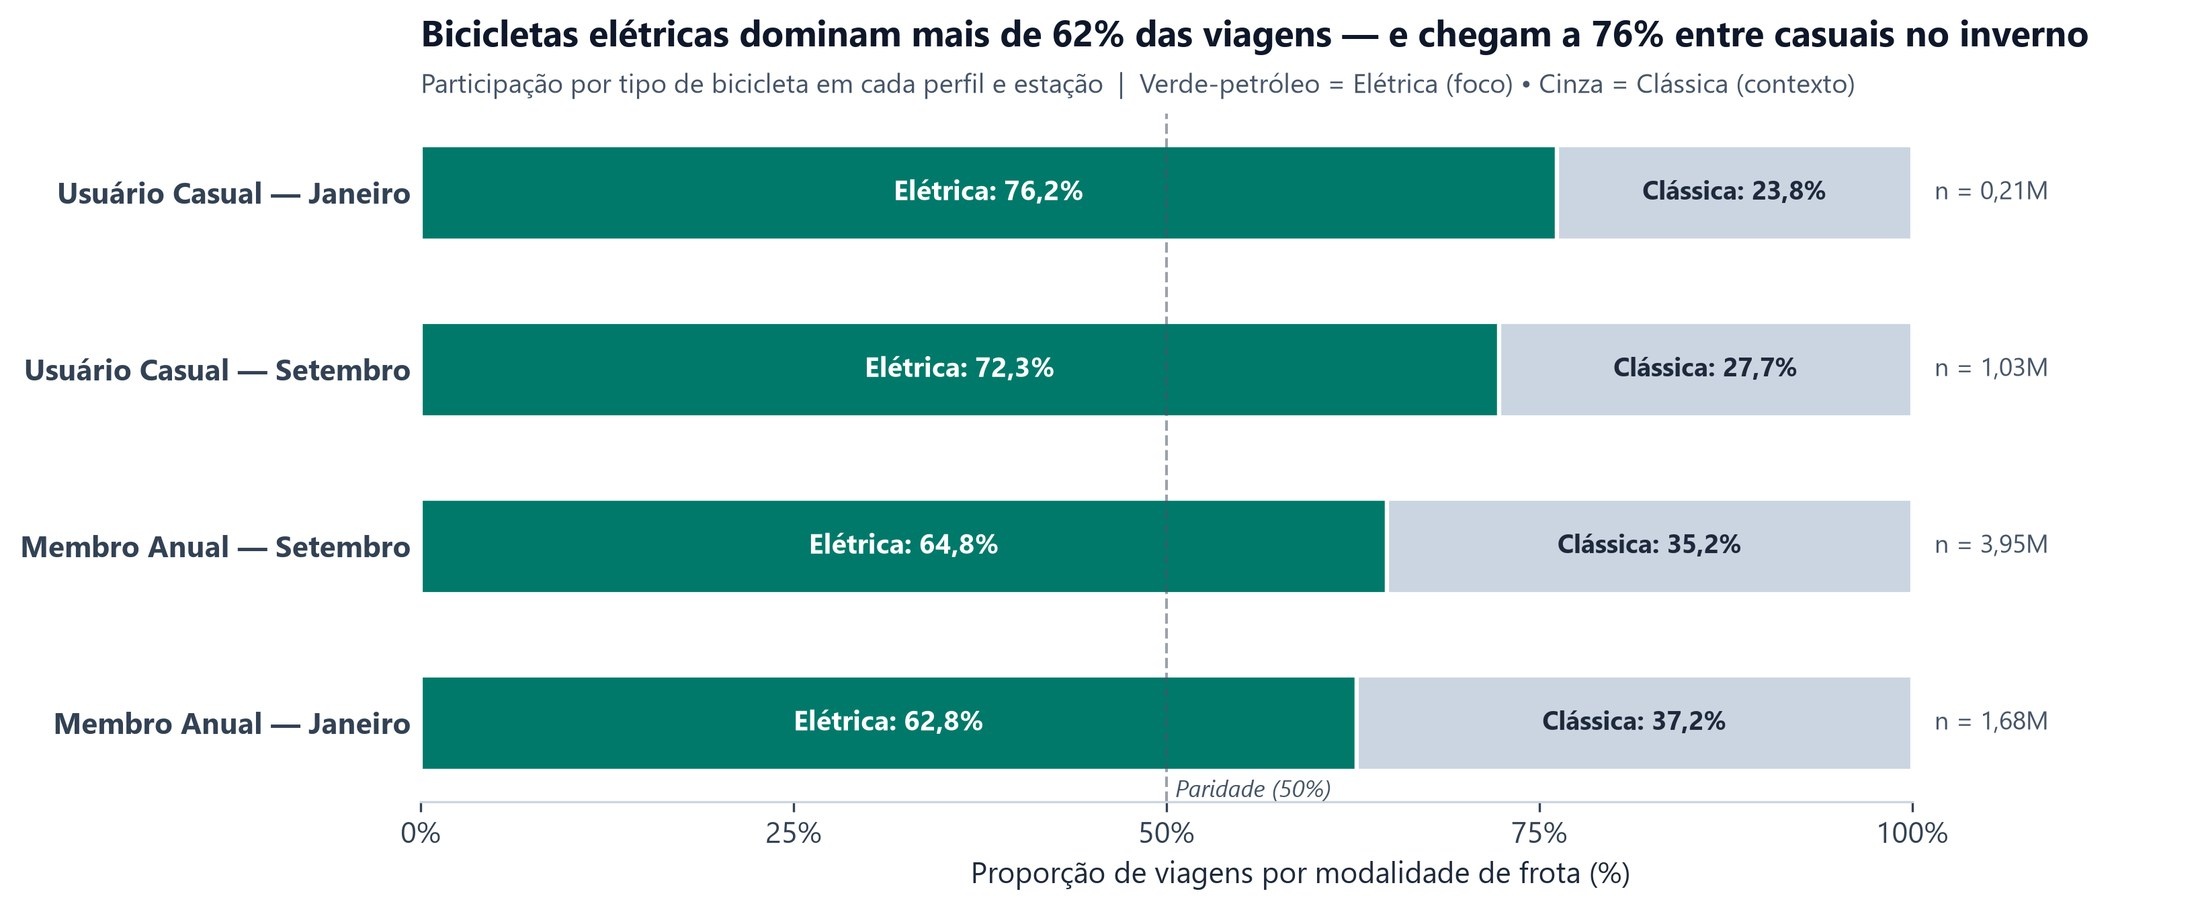
\includegraphics[width=0.8\textwidth]{rv2_preferencia_frota.jpg}
	\caption{Participação de bicicletas elétricas e clássicas por perfil e mês.}
	\label{fig:rv2}
\end{figure*}

\subsection*{Ritmo circadiano}

Nos dias úteis há dois picos agudos, às 8h e às 17h, típicos do deslocamento casa-trabalho. Fins de semana e feriados têm uma curva suave entre 12h e 17h, e a demanda de verão é 4,1 vezes a de inverno (Figura \ref{fig:rv3}). Feriados em dia de semana, como Ano Novo e Labor Day, eliminam o pico da manhã.

\begin{figure*}[t]
	\centering
	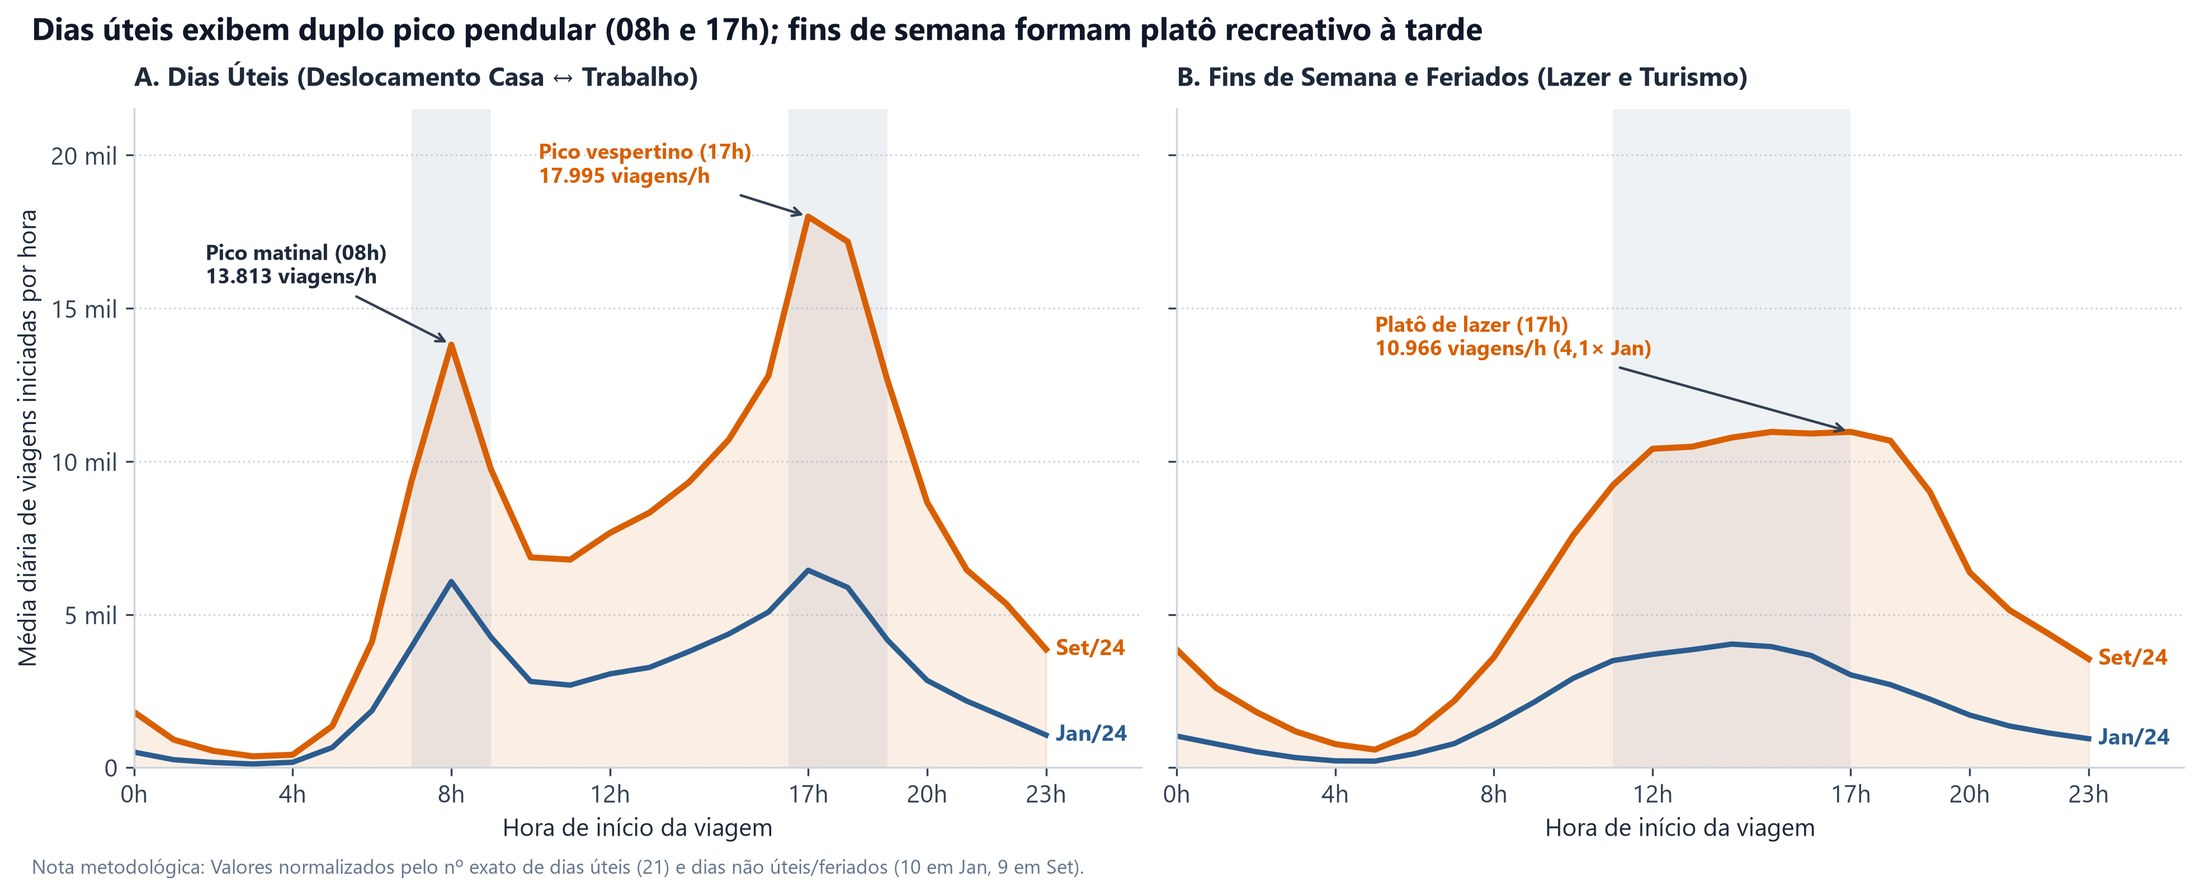
\includegraphics[width=0.9\textwidth]{rv3_ritmo_circadiano_demanda.jpg}
	\caption{Demanda horária média por dia, em dias úteis e em fins de semana e feriados.}
	\label{fig:rv3}
\end{figure*}

\subsection*{Duração das viagens}

A mediana dos membros é de 7,5 minutos em janeiro e 8,8 em setembro, compatível com o uso de última milha junto ao metrô. Usuários casuais pedalam cerca de 50\% mais (mediana de 13,2 minutos em setembro), mas a maioria encerra antes de 30 minutos (Figura \ref{fig:rv4}).

\begin{figure*}[t]
	\centering
	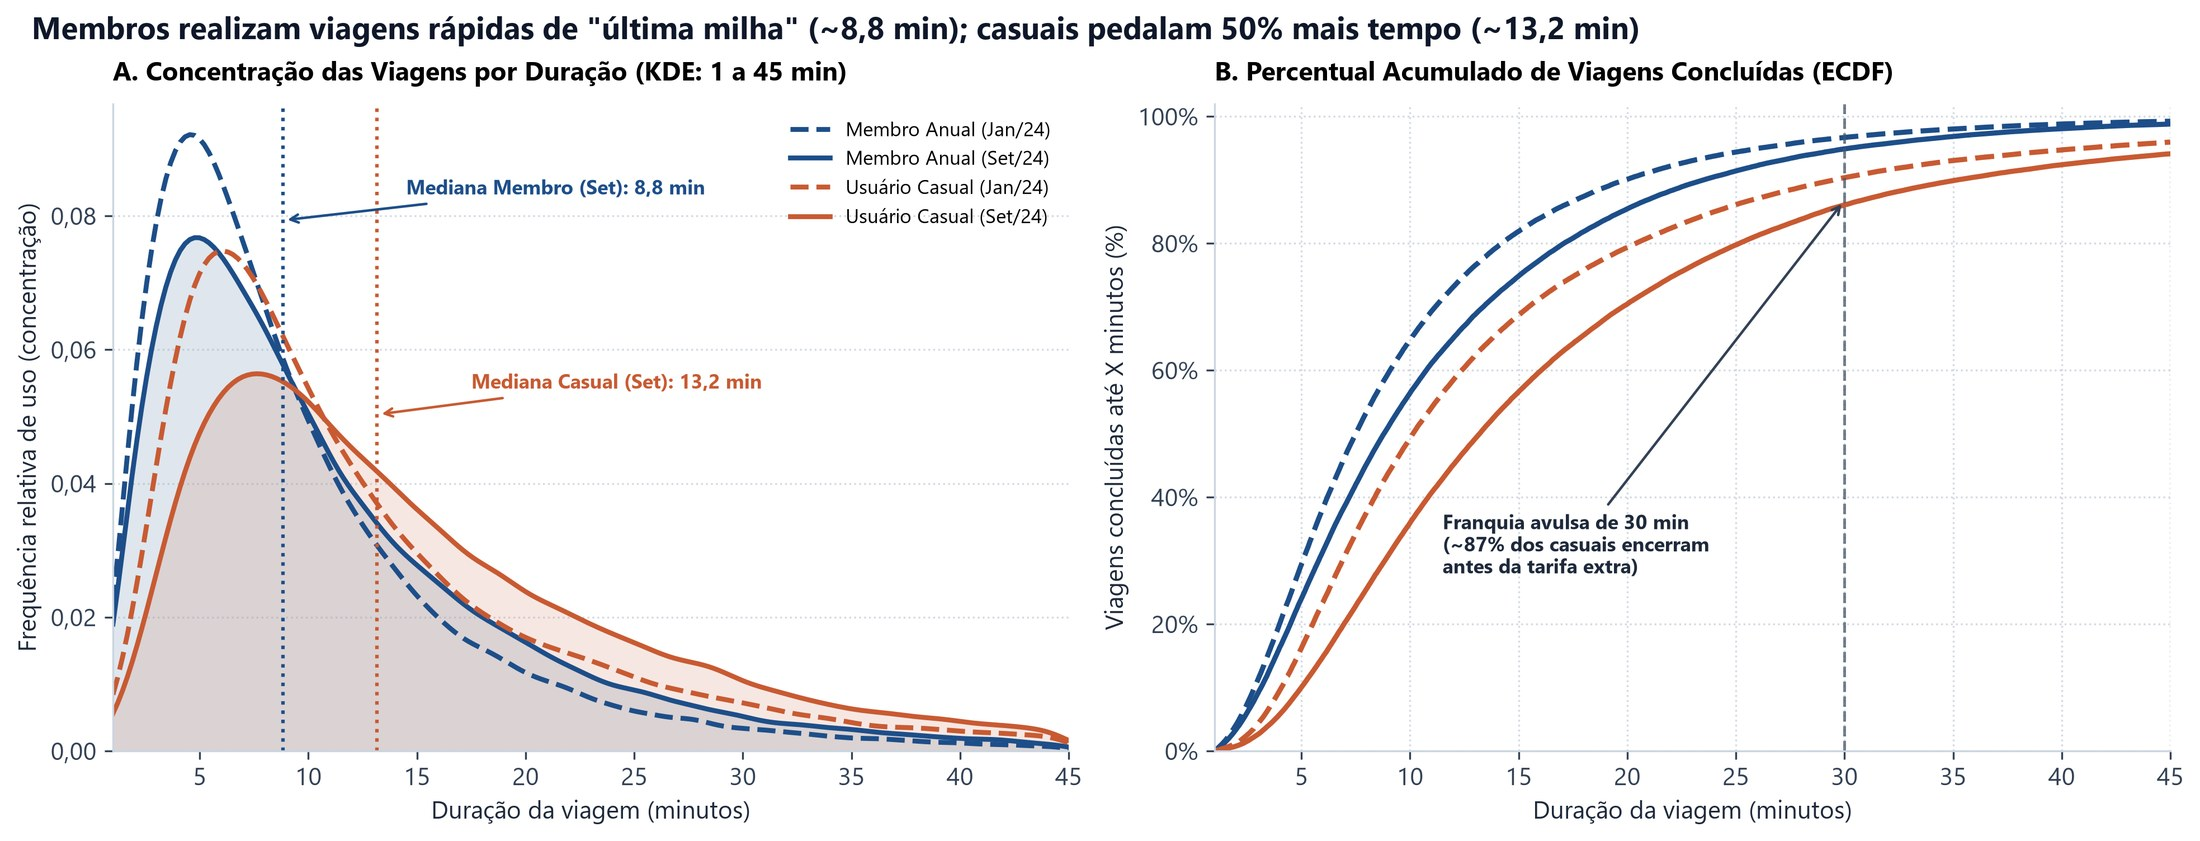
\includegraphics[width=0.9\textwidth]{rv4_distribuicao_duracao.jpg}
	\caption{Distribuição de duração (densidade) e percentual acumulado.}
	\label{fig:rv4}
\end{figure*}

\subsection*{Pêndulo geográfico}

Entre 7h e 9h, bairros residenciais (Upper West Side, Upper East Side, East Village e Williamsburg) têm déficit de bicicletas, enquanto Midtown e Financial District recebem mais do que enviam. Entre 17h e 19h o sentido se inverte (Figura \ref{fig:rv5}).

\begin{figure*}[t]
	\centering
	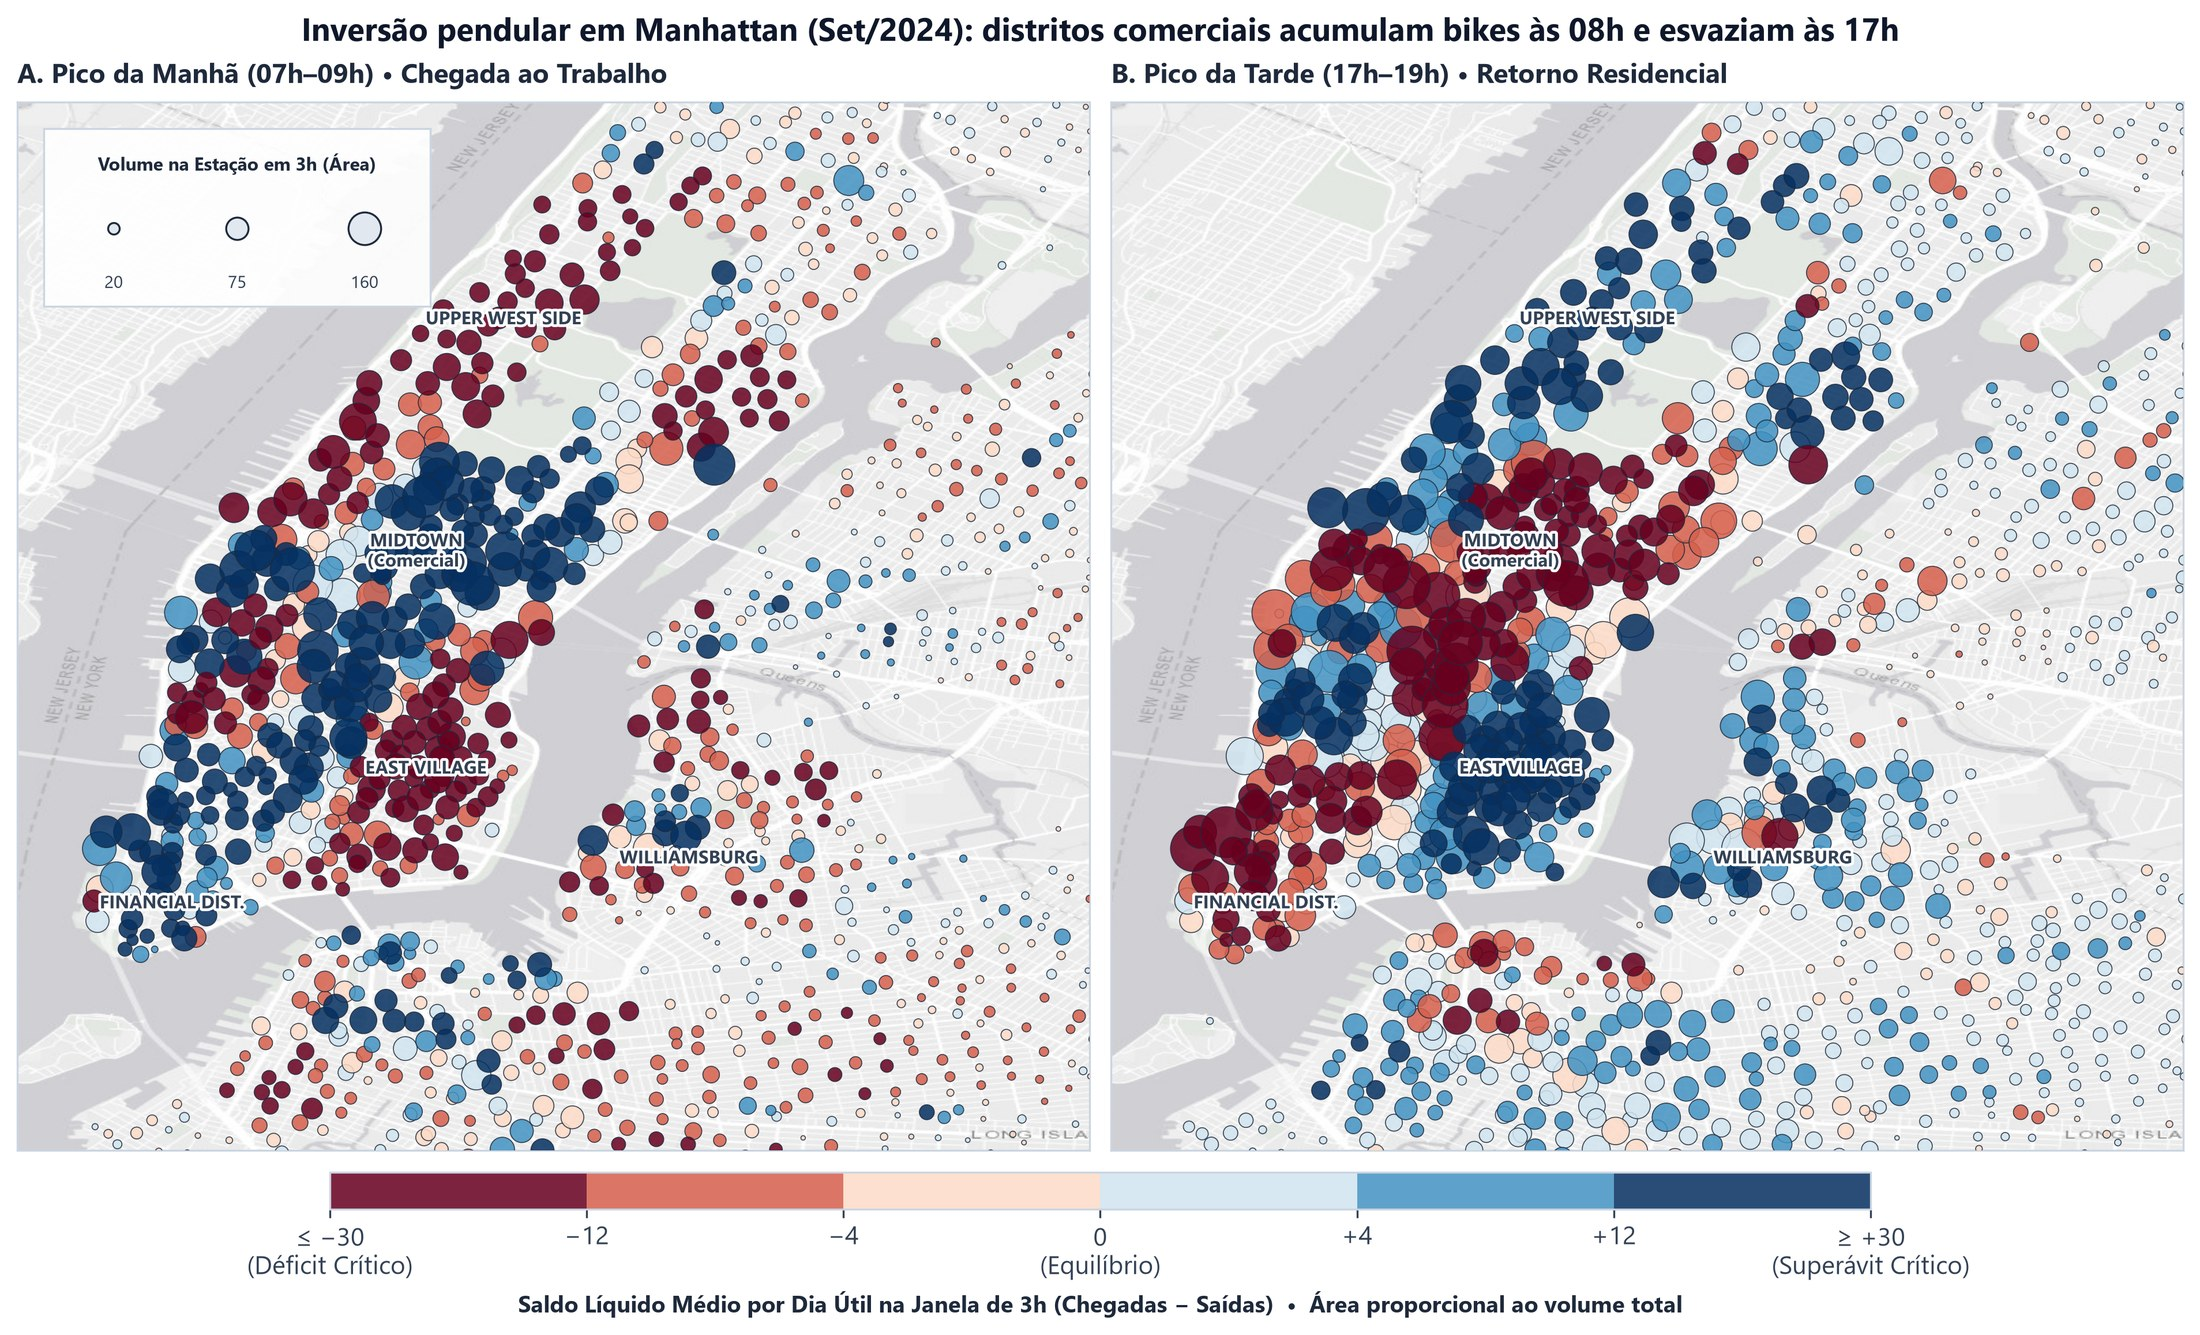
\includegraphics[width=0.75\textwidth]{rv5_assimetria_espacial_pendular.jpg}
	\caption{Saldo líquido (chegadas $-$ saídas) por estação, de manhã e à tarde. Vermelho indica déficit e azul, superávit.}
	\label{fig:rv5}
\end{figure*}

\subsection*{Animações}

Duas animações de 60 FPS, de uma semana de cada mês, mostram essa pulsação ao longo do tempo\footnote{\url{https://github.com/guirochasan/city_bike_analysis}}. Em janeiro, o fluxo cai cerca de 54\% no fim de semana de 6 e 7, após a primeira tempestade de neve do ano. Em setembro, o feriado de Labor Day tem padrão recreativo, seguido da explosão pendular dos dias úteis.

\section*{Conclusão}

O Citi Bike pedala no ritmo do trabalho, mas o verão traz o público casual e a frota elétrica. Os padrões sugerem três decisões: concentrar a manutenção pesada no inverno, garantir baterias carregadas em áreas turísticas e pré-posicionar bicicletas antes dos picos, usando calendário de feriados e previsão do tempo, e não apenas o dia da semana. Como limitações, usamos só dois meses de um ano; incluir mais meses e variáveis meteorológicas é o próximo passo.

%	REFERÊNCIAS
\printbibliography[title={Referências}]

\end{document}